\chapter{StreamIt Limitations and Proposed Extensions}
\label{section:impl_issues}

During the implementation process I encountered situations 
 where StreamIt forced a poor expression of a computation or 
language features did not scale for large application development. 
A language design oriented to small applications and benchmarks could easily 
miss these pragmatic development issues. The StreamIt group has focussed on 
these issues; 
the next version of StreamIt will add a number of language
extensions that improve programmability, modularity, 
and expression of parallelism and 
communication. 
This chapter provides concrete 
examples motivating
the introduction of these features and attempts to steer the direction of 
future streaming languages.

\section{Bitstream Parsing}

In MPEG-2, the process of parsing the bitstream and performing Huffman 
and run-length coding is estimated to constitute almost a third 
of the computational effort~\cite{iwata98coarse}. Unfortunately, many 
layers of nested control flow make the parser unsuitable for streaming 
computation. The parser must be implemented as a single filter that 
contains approximately one thousand lines of code, almost half the code 
lines in either the decoder or encoder. This filter expresses scheduling 
information and parallelism poorly. 

Filters with dynamic IO rates present particular difficulties for the 
StreamIt compiler because of the lack of scheduling information. However, 
certain filters are naturally expressed by the programmer with dynamic 
input and output rates, although they theoretically could 
be realized with static rates. 
In the decoder, the parser has a dynamic 
input rate, but always outputs full macroblocks, and ought to be expressed 
with a static output rate. (The reverse is true for the parser in the encoder.) 
However, due to the complexity of the MPEG-2 bitstream format, the actual 
push statements are embedded in deeply nested control flow. The parser is 
most naturally expressed in terms of a single work function execution 
that parses the entire MPEG-2 bitstream. 

This presents several difficulties. The fact that the parser processes all 
its data in a single pass means that if the filter were to execute atomically 
with respect to other filters, one would need a potentially infinite buffer 
between the parser and the downstream graph. To avoid this difficulty the 
compiler would need to generate multi-threaded code, even for a uniprocessor 
backend, that interleaves the parser execution with downstream execution. 
Messaging presents a second difficulty.
A filter's messaging granularity is determined by its input and output rates, 
and messages are timed with respect to the work execution boundaries; a work 
function that processed an entire video in a single execution could only 
time messages with respect to the beginning or end of the video, not with 
respect to individual macroblocks within the video.

I present a workaround that allows for interleaved scheduling and message 
delivery. Given a filter with a large work function, such as the parser, 
one can move control flow determining variables into filter instance 
variables that are maintained between work function executions. Inside 
the work function invocation is a loop that repeatedly branches to one 
of several helper functions determined by the control variables. The 
helper functions update the control variables, and the loop terminates 
after executing any of the helper functions that generates output (for 
the parser, pushing a macroblock). This workaround amounts to replacing 
nested control flow with a flat control flow graph structure. The 
readability and malleability of the code suffers. 

Even with such a hack, parallelism is expressed poorly because the parser 
itself cannot be parallelized easily. Two constructs in the MPEG-2 bitstream 
facilitate parser parallelism. At the higher level, every GOP can be decoded 
in parallel, since pictures can only reference other pictures in the same 
GOP. At a lower level slices may be decoded in parallel since macroblocks 
contained inside different slices in a picture are known to have no 
interdependencies. The codes for the start of a GOP or slice are 
byte-aligned and never occur in any other context. A parser exploiting
thread-level parallelism 
could first scan through a bitstream and identify the GOP and slice 
structures, and then subdivide portions of the bitstream to different 
bitstream parsers. Ahmad et al. show this technique to be 
effective for parallelizing MPEG-2~\cite{ahmadmpeg2encoder3}. 
This sort of parser parallelization is difficult to 
express in a stream based language and achieving reasonable performance 
would require a Herculean compiler effort.

The StreamIt group has considered language features to address these 
problems, but our key insight is the realization that StreamIt targets 
streaming computations, and if a filter cannot concisely express a 
computation then that computation is probably not streaming. For the MPEG-2 
parser this is obvious because its expression requires a thousand line 
functional block and leaves the compiler with an intractable parallelism 
problem. MPEG-2 bitstream parsing has little in common with stream 
computation and much in common with context-free grammars, and would be 
implemented more easily in a language like C. Clean interfaces between 
StreamIt and traditional languages, under development in the StreamIt 
language group, would allow hybrid language compression scheme implementations 
that share the benefits of both languages. MPEG-2 provides a strong motivation
for such a hybrid; while the majority of MPEG-2 coding is particularly well 
suited to a streaming approach, bitstream parsing is an important exception 
that demands an alternate approach.

\section{Functions with Tape Access}

Functions provide an abstraction that improves programmability when a computation 
must be repeated within a single work execution of a filter. Support for arbitrary 
tape accessing functions is a current focus of the StreamIt compiler group. A 
scheduler can handle both external and helper functions with tape access; the 
overall work rate of a filter should reflect any tape access caused by functions 
it calls. This section gives examples showing this feature's importance. 

\paragraph{External Functions with Tape Access}

\begin{figure}
  \begin{footnotesize} 
  \begin{center}
  \begin{minipage}{4.7in}
    \setlength{\columnseprule}{1pt}
    \begin{multicols}{2}
     \begin{minipage}{3in}
      \begin{verbatim}
...
int horizontal_size_value = 
  popbits(12);



int vertical_size_value = 
  popbits(12);



int aspect_ratio_information = 
  popbits(4);



int frame_rate_code = 
  popbits(4);



...
      \end{verbatim}
     \end{minipage} 

     \begin{minipage}{4in}
      \begin{verbatim}
 ...
 int horizontal_size_value = 0;
 for (int i = 0; i < 12; i++) {
   horizontal_size_value <<= 1;
   horizontal_size_value += pop();
 }
 int vertical_size_value = 0;
 for (int i = 0; i < 12; i++) {
   vertical_size_value <<= 1;
   vertical_size_value += pop();
 }
 int aspect_ratio_information = 0;
 for (int i = 0; i < 4; i++) {
   aspect_ratio_information += pop();
   aspect_ratio_information <<= 1;
 }
 int frame_rate_code = 0;
 for (int i = 0; i < 4; i++) {
   frame_rate_code <<= 1;
   frame_rate_code += pop();
 }
 ...
        \end{verbatim}
     \end{minipage}
    \end{multicols}
  \end{minipage}
  \end{center}
  \end{footnotesize}

  \caption{Code fragment from parser with (left) and without (right) tape accessing external functions.}
  \label{fig:mpegbitpopexample}
\end{figure}

Data compression formats such as JPEG and MPEG-2 pack data together as 
tightly as possible, ignoring word and byte boundaries in a data stream 
except for certain byte-aligned \textbf{escape codes} used to help a parser 
detect its position in a data stream. Even uncompressed formats, such as 
BMP~\cite{bmp} pack some configuration data. 
Parsers need functions that allow them to specify that a sequence of $N$ 
bits appearing in the bitstream should be consumed and stored as some data 
type, such as an integer. The left half of Figure~\ref{fig:mpegbitpopexample} 
shows example 
code from an MPEG-2 parser with external functions. The alternative approach 
without external functions appears in the right 
half\footnote{The particular ability to pop, 
push, and peek multiple bits at a time from (or to) bitstreams, as 
illustrated in this example, is needed so frequently that all of the 
implementations described in this paper assume that these global functions 
exist and must be preprocessed before being sent to the StreamIt compiler.}.

\paragraph{Helper Functions with Tape Access}
\label{sec:helperfunctionswithtapeaccess}
Helper functions with tape access allow for cleaner code. 
They differ primarily from external functions with tape access 
in that they would be private to the filter that contains them
and could manipulate internal state within that filter. 
The work function from the filter responsible for motion prediction
is 103 lines and is difficult to read or edit (the code is omitted due to length).
With tape-accessing helper functions it would decompose nicely into a work
function and three helper functions, each of 20 to 30 lines.

\section{Messaging Interfaces}
 
In the current version of StreamIt, a filter {\tt X} declares the types of messages 
it receives, and an associated {\tt portal<X>} is implicitly declared. Only filters 
of the same type may subscribe to the same portal, so redundant portals must be 
declared if different parts of a computation need the same sets of messages. The 
StreamIt group has recognized this limitation and the upcoming language revision 
will introduce messaging interfaces, conceptually similar to Java's interface 
declaration, that decouple portal specifications from subscriber implementations. 
An interface declares a set of valid messages, and any filter which implements the 
interface may subscribe to portals of the interface's type. 

Separating portal and subscriber definitions removes the dependency that senders 
broadcasting messages to a portal of type {\tt portal<X>} have on subscribers 
that implement \texttt{X}. This dependency limits the expression of large applications 
and I provide empirical evidence that motivates implementation efforts for this feature. 
Consider again 
Tables~\ref{table:enumerate_messages_decoder}~and~\ref{table:enumerate_messages_encoder}. 
The number of distinct message subscriber types demonstrates the need for interfaces.
Without interfaces, one must write each message sender after implementing all of its 
message receivers. In the encoder, enough components exchange information about picture 
and block metadata that message passing without interfaces became unmanageable and many 
parameters were embedded in the data stream. Interfaces enable one to write an MPEG-2 
bitstream parser before writing --- or even determining --- the many downstream 
components that will need to receive control parameters from the parser. 

\section{Programmable Splitjoins}
\label{sec:program_splitjoins}

The current language semantics support roundrobin and duplicate splitters, and roundrobin 
joiners. Roundrobin components need not send or receive identical amounts on each of their 
substreams, but the rates must be statically determined. Some applications require 
computations which dynamically switch between several modes of computation based on data. 
Messaging can address the issue when the modes of computation are very similar. However, 
in cases where the computations differ significantly, it would be more natural to place 
independent filters in parallel and have a splitter select one of the filters for each 
set of data to be processed. This provides a need for programmable splitters and joiners 
which can receive messages that determine the data streams to which they should output. 
I first give an example where some kind of \textbf{switch} splitter that sends to one of 
its channels would suffice, and then show a case where programmable splitters and joiners 
are needed.

\paragraph{Switch Splitjoins}

\begin{figure}[t]
  \begin{center}
    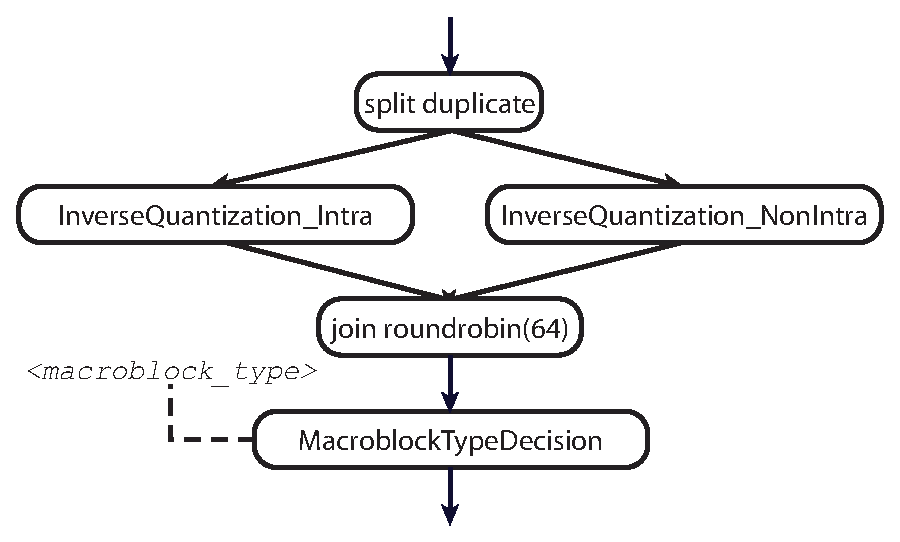
\includegraphics[scale=0.5, angle=0]{./inverse_quantization.eps}
    \caption{Inverse quantization subgraph with a duplicate splitter and roundrobin joiner.}
    \label{fig:inversequant}
  \end{center}
\end{figure}

\begin{figure}[t]
  \begin{center}
    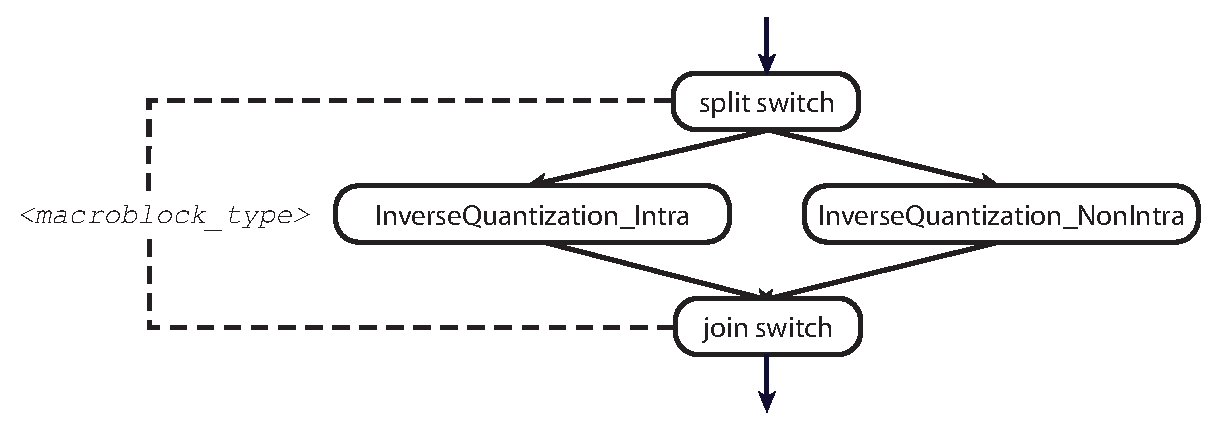
\includegraphics[scale=0.5, angle=0]{./inverse_quantization_switch.eps}
    \caption{Inverse quantization subgraph with switch splitters and joiners.}
    \label{fig:inversequant_switch}
  \end{center}
\end{figure}

Figure~\ref{fig:inversequant} shows the inverse quantization subgraph as it is realized in the 
MPEG-2 decoder. The inverse quantization process uses two different transforms depending on whether 
a block is intra coded or residually coded. The current implementation uses a splitjoin to 
duplicate each quantized block and process it for both block types. The results are interleaved 
and a downstream filter takes in both results and outputs one of them. Messages to the decision 
making filter from the upstream parser control which result gets output.

This approach results in needless computation since only one of the two intermediate filters 
needs to execute. Dataflow is also complicated by the interleaving and filtering of data. 
In this case, a paired switch splitter and joiner are desirable. The idea is that a switch 
splitter and joiner with coordinated behavior would receive messages which cause them to 
change which channel processes the data. Figure~\ref{fig:inversequant_switch} shows how the 
subgraph would appear with a switch splitter and joiner.

\paragraph{User Programmable Splitters}

Motion estimation in an MPEG-2 encoder, previously described in 
Section~\ref{encoder:estimation}, illustrates the need for a programmable splitjoin. As implemented 
in Figure~\ref{fig:motion_estimation_subgraph}, a duplicate splitter sends data to each of the 
compression filters. A roundrobin joiner interleaves each of the compression results and sends 
them to a downstream filter which determines the best encoding technique and emits only one of 
the compression results. However, this results in extra work. For I pictures one need not try 
motion estimation and for P pictures one need not try backward motion prediction. With only 
duplicate splitters and roundrobin joiners one is forced to send and receive data from the unneeded 
compression filters and then discard the results.

In an ideal implementation, the splitter and joiner would be 
programmable and messages about picture type would dictate which, 
and how many, internal streams processed the data. 
Figure~\ref{fig:motion_estimation_subgraph2} illustrates a stream 
graph with this form. A switch splitter will not suffice because 
multiple streams within the splitjoin must receive the input in 
certain cases. The joiner is also the ideal place to make the 
decision about which candidate blocks are used. For any given picture type, 
it must pop off the candidates from the valid input lines and output 
the one that exhibits the best compression. Note that the 
programmable splitter and joiners for this subgraph will be dynamic rates.
However, the motion estimation subgraph is still static rate with respect
to the rest of the stream graph and has a well-defined internal schedule.
I explain how this scheduling information can be exposed to the 
compiler in the next section.

\begin{figure}[h]
  \begin{center}
    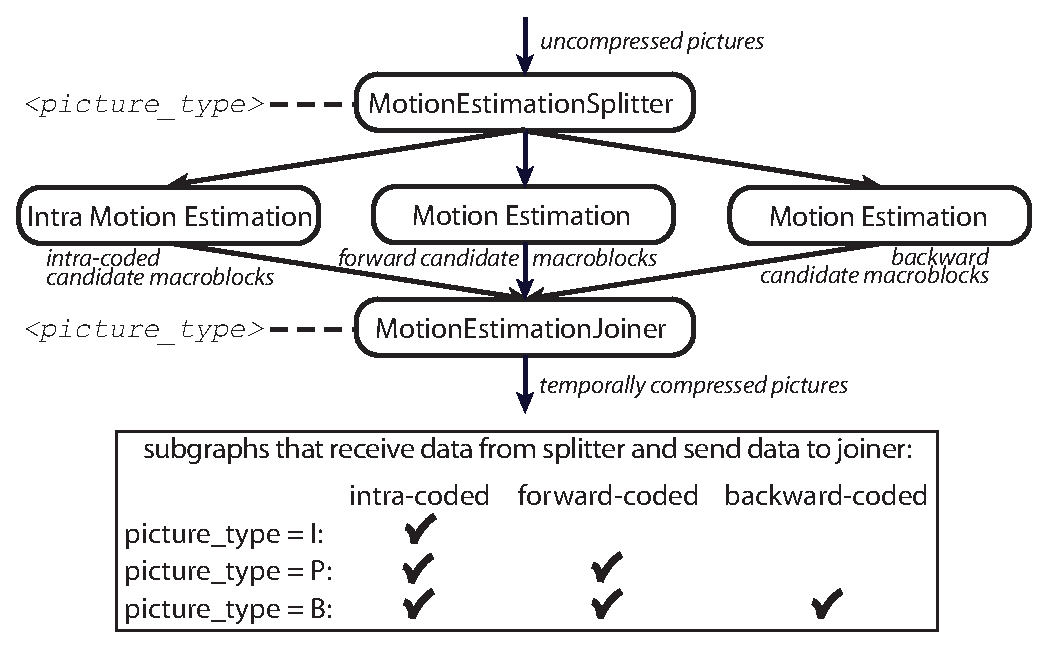
\includegraphics[scale=0.8, angle=0]{./motion_estimation_programmable.eps}
    \caption{Motion estimation stream subgraph with a programmable splitter and joiner.}
    \label{fig:motion_estimation_subgraph2}
  \end{center}
\end{figure}

Another part of the encoder that would benefit from programmable splitjoins
is the \texttt{ReferenceFrameHandler} responsible for decoding the 
recently encoded reference pictures and 
sending them upstream to the motion estimation filters. The subgraph
for this component appears in Figure~\ref{fig:referenceframe}.

\begin{figure}[h]
  \begin{center}
    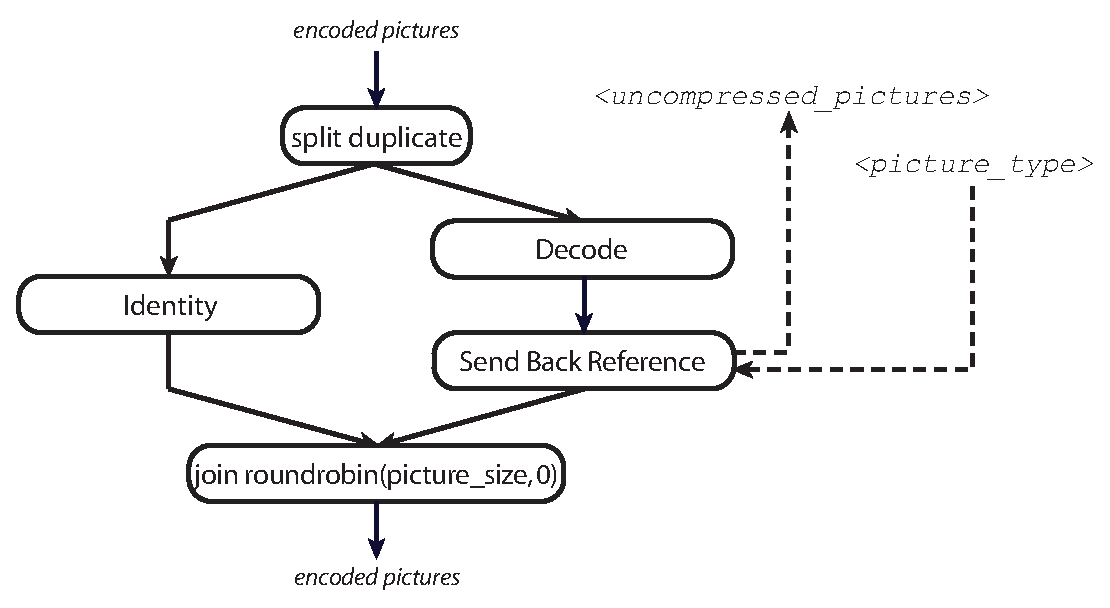
\includegraphics[scale=0.6, angle=0]{./referenceframe.eps}
    \caption{Subgraph for decoding reference pictures and sending them upstream.}
    \label{fig:referenceframe}
  \end{center}
\end{figure}

As currently realized, both reference pictures and non-reference pictures
go to a duplicate splitter. One duplicate of the encoded picture passes back 
to the joiner unchanged, and the other goes to a subgraph that first
decodes the picture and then sends it as an upstream message
to the motion estimation filters. The subgraph for decoding the picture
looks similar to the MPEG-2 decoder pipeline.

One problem with this behavior is that the filter responsible for messaging
back the reference frame must determine whether or not to send the 
picture or merely discard it, based on the picture type. This is
problematic because many pictures are discarded, yet they are still properly
decoded. A programmable splitter 
could receive picture type messages and selectively send only the 
reference frames to the decoding subgraph. This would avoid
unnecessary computation.

\section{Named Work Functions}

Many filters whose work function behavior is dependent on stream parameters 
have a similar implementation pattern: state variables are declared and are 
used as parameters or control flow indicators in the work function, and only 
ever modified in message updates. 

A more intuitive mechanism for the programmer 
would be to allow multiple named work functions or a single named work 
function that declares parameters (like a function or filter 
declaration). These named work functions would act as message receivers, and 
other portals could directly call the work functions through the teleport 
messaging mechanism. 

From a sending filter's standpoint, messaging is unaffected.
Whether a receiver implements a message handler as a 
named work function or a message handler is irrelevant to the messaging semantics. 
When a filter with a named work function receives a message, 
it would change the filter's mode of execution to the named work function,
using the work function parameters if they exist.

Using named work functions simplifies the programming of the quantization, motion 
estimation, and picture reordering filters in the encoder, and the inverse 
quantization and motion prediction filters in the decoder. 
This feature also makes filter behavior more transparent to the compiler
by exposing scheduling information about otherwise dynamic rate components. 
For instance, some dynamic rate filters could be declared as static rate filters
if the different named work functions had different pop and push rates.

As an example, I consider the MPEG-2 encoder's motion estimation 
subgraph realized using programmable splitters and joiners, previously
described in Section~\ref{sec:program_splitjoins}. As 
Figure~\ref{fig:motion_estimation_subgraph} points out, the splitter
and joiner will need to have different IO rates depending on the 
picture type, because different numbers of the splitjoins
internal streams may need to receive picture data.
With dynamic splitter and joiner IO rates, a compiler would be unable to 
intelligently schedule the subgraph's execution.

Suppose the splitter and joiner could each be implemented using 
three named work functions. Each work function would have a different but
static rate declaration. By sharing the same interface and subscribing
to the same message portal, this would expose the scheduling information
to the compiler, which could realize that the splitjoin viewed as a whole
has a static IO rate with respect to the rest of the graph. 

\section{Stream Graph Reinitialization}

The biggest limitation of StreamIt 2.0 codec implementations
is a requirement placed on video and image parameters that determine 
stream graph topology. These parameters must be declared at compile-time. 
Image size and chroma format must be hardcoded and changes to these values 
require that the source code be modified and the program recompiled. 
This limitation can be removed by allowing portions of a stream graph 
to reinitialize at runtime. Others have had success allowing actors to
reinitialize at runtime and change their internal 
state~\cite{neuendorffer04hierarchical}, and it should be possible
to allow topology changes at runtime as well. I believe this language
feature is necessary  and the StreamIt group is introducing the ability
in StreamIt 3.0.

\section{Stream Graph Draining}

The streaming model of computation assumes that input and output streams are infinite 
and actors will process continuously with a steady state behavior. However, real 
world applications such as MPEG-2 have definite stream endings, and the end of life 
behavior of a stream graph is poorly determined. The MPEG-2 decoder, for instance, 
needs to be \textit{drained} so that filters internally buffering data release their 
buffers. An example of this is the filter responsible for picture reordering 
(previously shown in Figure~\ref{fig:picture_reorder}) which buffers one reference frame 
internally. For this frame to get released, the current implementation requires that 
the first filter in the pipeline, after detecting its final input, send dummy data 
items through the pipeline to empty out the remaining buffers. However, this behavior 
is non-ideal because spatial and temporal decoding are performed on data whose only 
purpose is to cause the downstream filter to release buffered data items. Just as 
the \texttt{prework} keyword helps a stream-graph reach a steady-state behavior at 
application startup, a similar mechanism (e.g., \texttt{postwork}) is needed at the 
end of an application's lifetime.